%=============================================================================
% Thesis Template in LaTex
%
% File: 04-08-Risiken - Bewertung der Lösung -- Fallstudie
% Author(s): Jürgen Hackl <hackl@ibi.baug.ethz.ch>
%            Clemens Kielhauser <kielhauser@ibi.baug.ethz.ch>
%
% Creation:  27 Jan 2014
% Time-stamp: <Tue 2013-08-13 20:14 juergen>
%
% Copyright (c) 2014 Infrastructure Management Group (IMG)
%               http://ibi.ethz.ch
%
% More information on LaTeX: http://www.latex-project.org/
%=============================================================================

% Unterkapitel Risikenberechnung 
% ---------
\label{subsec:BerechnungRisiken}


Wie im vorangegangen Abschnitt erwähnt, berechnet sich das Risiko einer Varianten in einem Szenario, durch die Multiplikation der Eintrittswahrscheinlichkeit des Szenarios mit den für die jeweilige Variante, im betrachteten Szenario, berechneten Kosten. Das Gesamtrisiko das von der Durchführung einer Variante ausgeht, setzt sich somit aus der Summe aller Risiken einer Variante zusammen. 
Anhand der nachfolgenden Abbildung wird als Beispiel die Berechnung des Risiko der Variante 1, mithilfe eines Entscheidungsbaums gezeigt. Die Berechnung erfolgt in diesem Fall von Rechts nach Links.


\begin{figure}[h!]
	\centering
	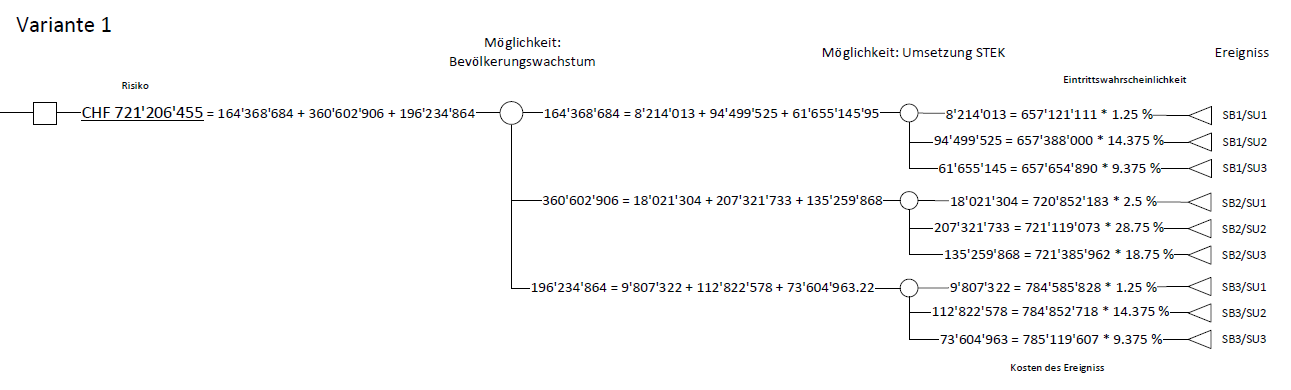
\includegraphics[width=\textwidth]{figures/f-04-08-01-Risikoberechnung}
	\caption[Risikoberechnung]{Beispiel der Risikoberechnung}
	\label{img:Risikoberechnung}
\end{figure}




% ===========================================================================
% EOF
%

%%% Local Variables:
%%% mode: latex
%%% TeX-master: "../main"
%%% End:
